\chapter{针对新一代视频编码标准HEVC的解码优化}

\section{引言}

新的视频编码标准HEVC虽然显著提高了编码效率,但其复杂度也有了明显的提升。现有的用户设备计算资源有限,如何快速实时的解码成为了HEVC广泛应用于流媒体系统的一个阻碍。在硬件解码芯片普及之前,软件解码器的实现和优化是一项重要且有挑战性的工作。在本章中,我们给出了一个高度优化的HEVC软件解码器,并对其在不同处理器平台上的速度进行了测试。

\section{新的解码器原型及框架设计}

HEVC标准化组织提供的参考软件HM中包含了一个HEVC解码器的实现。但是这个实现主要目的是为了方便标准制定和相关的研究工作,其结构冗余复杂,解码效率低下,不适合实际使用。为了确保本文后续优化工作的有效性和实用性,我们自行设计了一个新的解码器原型。

\begin{figure}[t]
	\centering
	\includegraphics[width = 1.0\linewidth]{figures/Decoding-Workflow.pdf}\\
	\caption{\label{fig:decoding_workflow}新的解码器原型流程框架}
\end{figure}

该解码器原型的四阶段流程框架如图\ref{fig:decoding_workflow}所示,其中列出了解码器结构中的四个关键阶段,即:高层语法解码、slice解码、CTU解码循环和CTU解码,对应图中的S1-S4。这个解码器原型有两个不同于HM中参考解码器的特性。第一,在CTU解码(S4)的开始阶段,数据会从全局性的帧缓冲区拷贝一份到CTU缓冲区。这样可以保持这个CTU解码过程中数据访问的局部性,从而降低处理器的缓存失效率。该特性有助于接下来要讨论的SIMD优化算法。第二,在CTU解码循环(S3)中,去块滤波和SAO这些理论上要等整帧解完之后才进行的操作,会在每个CTU的像素重建之后立即开始。这样使得这个CTU能够尽早被参考,也就意味着更多的解码任务可以并行执行。该特性为本文后面要介绍的帧级多线程解码框架打下了基础。

需要指出的是,虽然第一个特性有助于提高缓存命中率,但增加了数据拷贝的额外开销。为了尽量减小这一开销,我们会严格选择所需数据:对于当前的CTU解码,只有它上面和左边的CTU可能被用到;而且这两个CTU中有用的分别只是下边界和右边界的数据。按需进行精细复制可以避免大量多余的内存拷贝操作。另外的内存优化还包括对帧缓冲区的处理。所有帧缓冲区都被设计为全局的,只在解码程序开始时统一分配,解码过程中以内存池的方式进行管理,程序运行结束后统一释放。这一机制尽量避免了频繁地内存分配和释放操作,有利于提高程序的内存使用效率和执行速度。

在这一全新的解码器原型基础上,我们接下来用SIMD优化和多线程并行这两种方法来对整个解码过程进行加速。

\section{各个耗时模块的SIMD优化}

大多数现代通用处理器都有SIMD扩展指令集,例如x86架构上的MMX、3DNow!、SSEx、AVX等\supercite{Intel-manual},以及ARM架构上的NEON\supercite{ARM-manual}。这类指令集中的一条指令可以同时操作位于特殊向量寄存器中的多个数据,能成倍地提高数据吞吐率。在这一节中,我们用SIMD技术来优化HEVC解码中的几个耗时模块。

根据对HEVC复杂度的分析\supercite{Bossen-TCSVT2012,Yan-VCIP2012},解码中耗时较多且适合用SIMD来优化的几个模块包括:运动校正、变换、去块滤波和采样自适应偏移(SAO)。其中运动校正和变换已经在Yan等人的工作\supercite{Yan-VCIP2012}中被充分地优化过了,本文直接采用其结果。而对于已有工作尚未很好处理的去块滤波和SAO,我们将分别设计新的算法对其进行加速。下面介绍的算法对x86架构和ARM架构都适用,在具体实现上有差异的地方我们会单独指出。

\subsection{对称去块滤波算法}

在HEVC的去块滤波中,对于8x8的块边界,每次以4个像素为单元来决定是否需要进行滤波,并决定是进行高强度滤波还是普通滤波。这样就把边界同一侧每次操作的像素个数限制为4,无法充分利用向量寄存器同时对8个像素进行计算。为了提高并行度,我们设计了一个与Yang等人在H.264/AVC解码器优化工作\supercite{Yang-TCE2006}中的描述类似的对称去块滤波算法。

\begin{figure}[h]
	\centering
	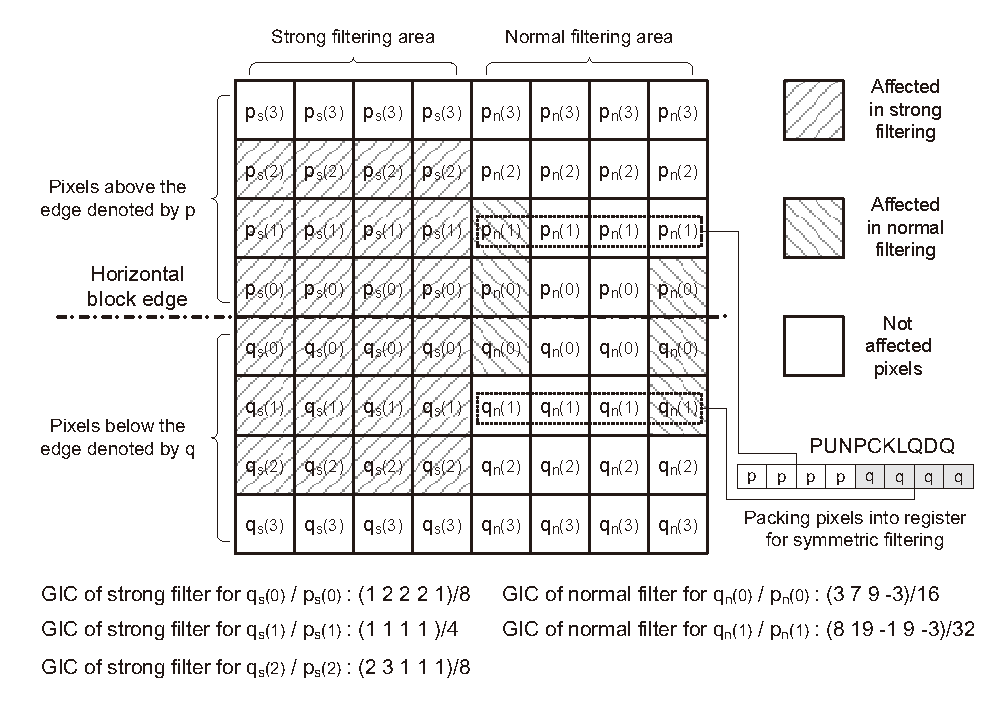
\includegraphics[width = 1.0\linewidth]{eps/vertical_DF_to_horizontal_edge}\\
	\caption{\label{fig:vertical_DF_to_horizontal_edge}HEVC中对$8 \times 8$块的水平边界进行滤波的操作示意图}
\end{figure}

图\ref{fig:vertical_DF_to_horizontal_edge}展示的是HEVC标准中对8x8块的水平边界进行滤波的操作示意图。滤波操作实质上就是对边界两侧的像素进行修改。在每侧的4个像素中,高强度滤波会修改其中的3个,普通滤波会修改其中的2个或1个或0个。修改的方法可以认为是一个插值的过程。原来的像素会被改为用它上下的像素进行插值(加权平均)的结果,从而实现像素值的平滑,达到消除边界的目的。在图\ref{fig:vertical_DF_to_horizontal_edge}所示的例子里,左边四列像素进行的是高强度滤波,右边四列是普通滤波。图的下方列出了对各个像素进行修改时用到的插值系数组(group of interpolation coefficients,简称GIC),相当于滤波器的冲激响应\supercite{Norkin-TCSVT2012}。这里有一个比较关键的地方在于,根据HEVC对滤波模块的规定,边界两侧相同位置的像素,其GIC是一样的,而且插值所用的像素也是对称的。利用这个性质,我们可以用PUNPCKLQDQ这一SIMD指令把边界两侧相同位置的像素放在一个寄存器里同时参与计算。如图\ref{fig:vertical_DF_to_horizontal_edge}中所示,在高强度滤波中,对于0~3的每一个$i$,标记为$p_n(i)$的4个像素和标记为$q_n(i)$的4个像素放在一起;同样的,在普通滤波中,对于0~3的每一个$j$,标记为$p_s(j)$的4个像素和标记为$q_s(j)$的4个像素放在一起。这样,无论是哪种滤波方式,每次能处理8个像素,充分利用了128位向量寄存器(在滤波操作中因为要存储中间值,每个像素需占用16位),使得滤波操作所需的指令数减少了一半。

对于普通滤波方式来说,因为受影响的像素数不确定(0个到2个),所以在与高强度滤波同样的方式计算出滤波结果之后,还要另外用某种阈值来决定哪些像素最终会被滤波结果取代。这时可以用阈值来构造掩模,用掩模去选择最终结果。例如,对于图\ref{fig:vertical_DF_to_horizontal_edge}中的$q_n(0)$和$p_n(0)$行,中间两个像素不受影响,所以其4 x 16bit掩模应为:
\begin{equation}
Mask = \{ \texttt{0xffff}, \quad \texttt{0}, \quad \texttt{0}, \quad \texttt{0xffff} \}.
\end{equation}
基于此,普通滤波的最终结果可确定为:
\begin{equation}
ResultRow = (OriginalRow \land \neg Mask ) \lor (FilteredRow \land Mask).
\end{equation}
这些操作可以用并行逻辑运算指令PAND、PANDN以及POR很轻易地实现。

上面讨论的是水平边界的滤波。对于竖直边界,该算法过程是一致的,只需要先进行一次转置,然后按照上述方法进行计算即可。

\subsection{并行索引SAO算法}

在HEVC解码中,去块滤波之后的像素需要先进行采样自适应偏移(SAO)才能输出为解码图像。对于每个CTU,其像素进行SAO的模式由码流中解析出的\textit{SAOType}来指定。SAO模式有两种,一个是条带(Band)模式,一个是边缘(Edge)模式。这两种模式都会在原像素值上增加一个偏移量。不同之处在于,在条带模式中,这个偏移量由原像素值本身(0~255)来索引,而在边缘模式中,这个偏移量由原像素与其两个相邻像素的梯度值来索引。在条带模式中,每个条带横跨的像素值为4,因此256个不同像素值被分为了32个条带,作为索引去查表决定加到该像素上的偏移量。这样的索引操作在ARM架构上可以用NEON指令集扩展中的并行查表指令进行优化。然而遗憾的是,x86架构下没有对应的指令,只能用普通代码实现。相比于条带模式,边缘模式则更为复杂。本节提出的并行索引SAO算法也主要是针对边缘模式。下面详细介绍。

在边缘模式中,一个像素要减去与它相邻的两个像素。这两个邻居所在的方向可以从图\ref{fig:SAO_edge_direction}中的四个方向选择其一。相减得到两个差值,差值根据其正负或0对应到1、-1和0这三个符号;将两个差值对应的符号相加(可能的结果为-2、-1、0、1、2),作为偏移量的索引。因为一个CTU中的所有像素相减方向都相同,所以计算索引的操作可以并行执行。对于128位的向量寄存器来说,一次可以处理16个像素。图\ref{fig:SAO_edge_parallel_index}展示了我们设计的并行索引算法的核心过程,其中用一对PCMPGTB/PCMPLTB指令和一对PAND/POR指令得到了16个像素相减的符号值。根据选定的方向求出两组符号值之后,通过PADDB指令将它们相加就得到16个索引值,最后用一条PSHUFB指令来查表得到所需的偏移量。很明显这种并行索引SAO算法已经取得了最大的数据级并行度,指令数量已经压缩到最少。需要指出的是,对于图\ref{fig:SAO_edge_direction}中$0^\circ$、$45^\circ$和$135^\circ$这三个方向的相减,将正确的像素取到向量寄存器中会有无法避免的开销,因为要访问的内存是非连续的。

\begin{figure}[!tp]
	\centering
	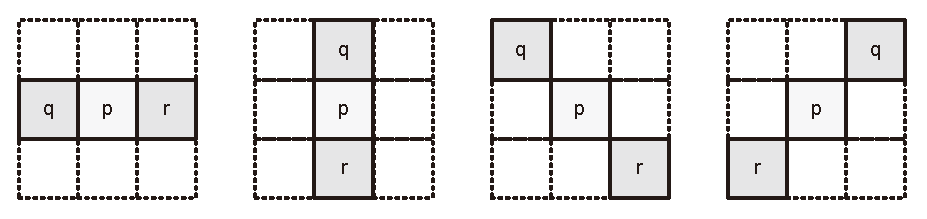
\includegraphics[width = 0.9\linewidth]{eps/SAO_edge_direction}\\
	\caption{\label{fig:SAO_edge_direction}HEVC中的SAO在边缘模式下选取相邻像素的4种方向}
\end{figure}

\begin{figure}[!tp]
	\centering
	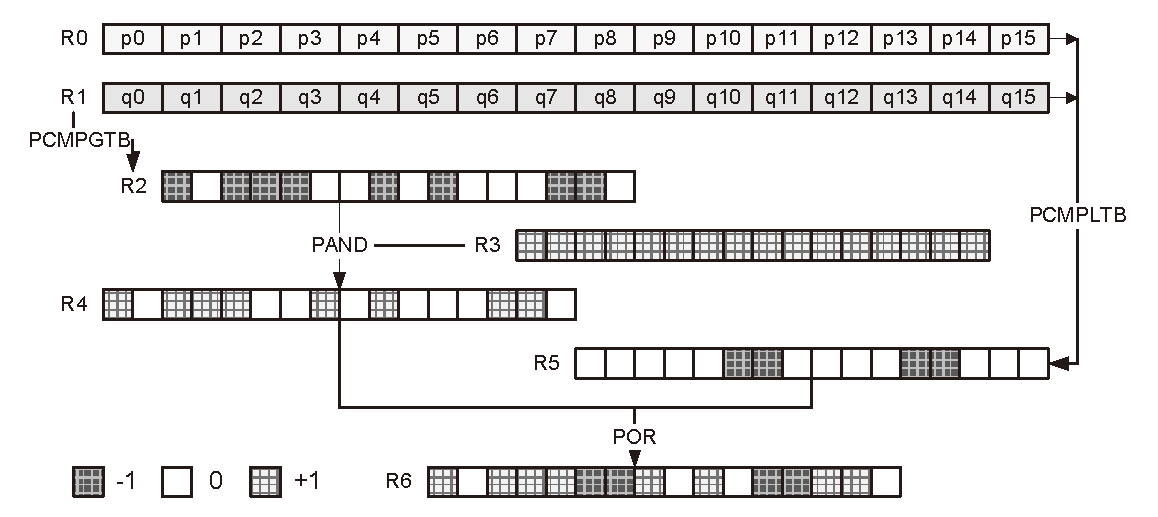
\includegraphics[width = 0.95\linewidth]{eps/SAO_edge_parallel_index}\\
	\caption{\label{fig:SAO_edge_parallel_index}HEVC中的SAO在边缘模式下的得到16个符号值的过程}
\end{figure}


\section{帧级并行解码}

本文提出的帧级并行解码框架如图\ref{fig:parallel_decoding_framework}所示。

\begin{figure}[!tp]
	\centering
	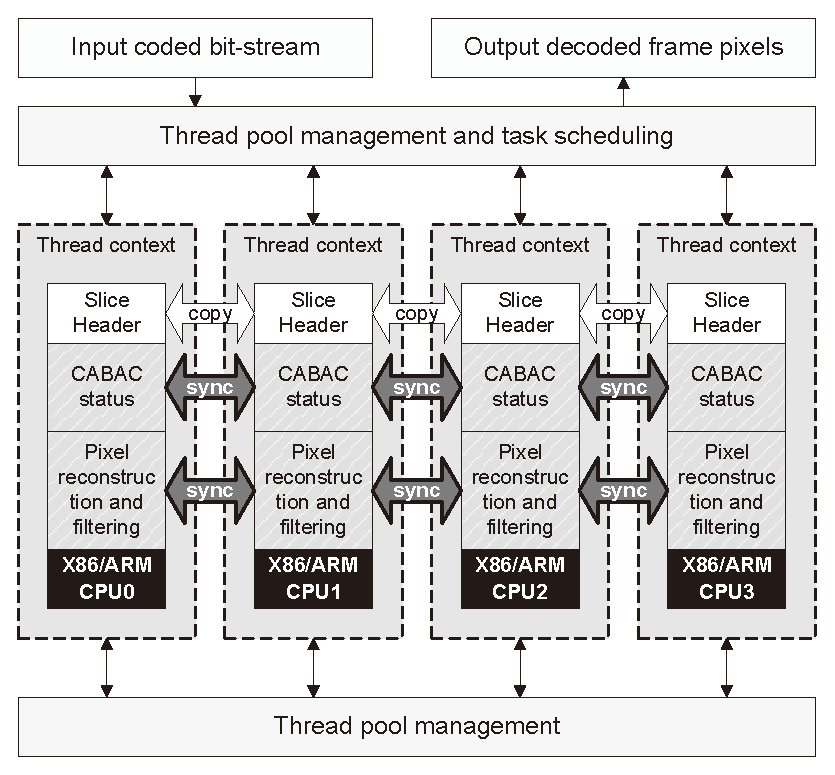
\includegraphics[width = 0.9\linewidth]{eps/parallel_decoding_framework}\\
	\caption{\label{fig:parallel_decoding_framework}HEVC帧级并行解码框架图}
\end{figure}

\section{优化结果}

\section{本章小结}









